\documentclass[conference]{IEEEtran}

\usepackage[utf8]{inputenc}
\usepackage[english]{babel}
\usepackage{graphicx}
\usepackage{float}
\usepackage{hyperref}
\usepackage{booktabs}
\usepackage{array}
\usepackage{amsmath}

\usepackage{tikz}
\usetikzlibrary{shapes.geometric, arrows.meta, positioning, fit, backgrounds}

\hypersetup{
    colorlinks=true,
    linkcolor=blue,
    urlcolor=blue,
    citecolor=black
}

\begin{document}

\title{Smart Campus Energy Management System: A Software-Defined Approach}

\author{
\IEEEauthorblockN{Omar Yesid Fonseca López, Daniel Felipe Barrera Suárez, \\ Daniel Mateo Ballesteros Molina, Dania Lizeth Guzmán Triviño}
\IEEEauthorblockA{\textit{Systems Engineering Program} \\
\textit{Universidad Distrital Francisco José de Caldas}\\
Bogotá, Colombia \\
\{oyfonsecal, dfbarreras, dmballesterosm, dlguzmant\}@udistrital.edu.co}
}

\maketitle

\begin{abstract}
High energy consumption in university facilities, primarily driven by unoccupied laboratories with active computing equipment, presents a critical sustainability challenge constrained by strict institutional IT security policies. To address this issue, we propose the design of a decentralized, software-defined Proof of Concept (PoC) that employs autonomous telemetry agents in the user-space, cloud data storage, and behavioral deterrents (nudges). The preliminary analytical review and architecture design demonstrate that this approach bypasses the need for physical IoT infrastructure or administrative privileges, providing a highly feasible, secure, and scalable solution to mitigate institutional waste.
\end{abstract}

\begin{IEEEkeywords}
Systems Analysis, Energy Management, Autonomous Telemetry, Smart Campus, Software-Defined.
\end{IEEEkeywords}

\section{Introduction}
Efficient energy management in higher education institutions has become a vital field of study due to its profound impact on operational efficiency and environmental sustainability. Previous studies demonstrate that university buildings exhibit critical levels of electricity consumption, where computing equipment in standby mode and lighting systems represent a constant source of waste \cite{b1, b4}. In addition, various researchers highlight that occupant behavior is a determining factor in building energy inefficiency, sometimes increasing consumption by up to 150\% \cite{b2}, which introduces an undeniable socio-technical dimension to the problem \cite{b3}.

Conventionally, approaches to mitigate this phenomenon have focused on physical energy audits under standards like ISO 50001 or the deployment of Internet of Things (IoT) sensor networks for infrastructure automation \cite{b2, b5}. However, in public university contexts, these physical interventions face nearly insurmountable logistical, budgetary, and bureaucratic barriers. Institutional Information Technology (IT) policies strictly prohibit the deployment of private perimeter networks, the use of third-party centralized orchestration servers, or the installation of software requiring administrator (\textit{root}) privileges on student workstations.

Faced with the technical impossibility of implementing traditional hardware-based solutions, this paper introduces a Software-Defined Energy Management approach. The core innovation of this project lies in shifting the monitoring intelligence from the physical infrastructure to the logical layer of the operating system by executing non-privileged scripts in the user-space. This solution seeks to align the campus's sustainability goals with rigorous cybersecurity policies, intervening in the human factor through behavioral deterrent techniques and implementing automatic, low-impact energy conservation mechanisms.

\section{Methods and Materials}
The development of the solution was based on a two-stage engineering process, combining primary data collection in the field with the design of a restrictive software architecture. In the first stage, the systems analysis was carried out in the laboratories of the Engineering Faculty at Universidad Distrital. Three non-invasive techniques were triangulated: direct observation of the spaces to quantify waste, correlation of ambient light levels using lux meters to evaluate daylight harvesting, and the application of structured surveys to 35 users to understand the role of human memory regarding energy-saving protocols.

The findings of this diagnostic phase confirmed a strong behavioral inertia; an overwhelming majority of users considered energy saving important but admitted forgetting to turn off equipment at the end of their lab sessions. Table \ref{tab:observation} illustrates a sample of the direct observation records, evidencing the recurrence of unoccupied laboratories with active computers and lighting systems during working hours. This phenomenon demonstrated that manual control was insufficient and an automated intervention was required.

\begin{table}[htbp]
    \centering
    \caption{Excerpt of Data Collected by Direct Observation}
    \label{tab:observation}
    \begin{tabular}{|c|c|c|c|c|}
        \hline
        \textbf{Date / Time} & \textbf{Space} & \textbf{Occupied?} & \textbf{Lights?} & \textbf{Active PCs?} \\
        \hline
        23-Feb 09:00 & Room 202 & No & No & N/A \\
        23-Feb 13:00 & Room 301 & No & Yes & N/A \\
        24-Feb 18:00 & Lab 500 & No & Yes & Yes \\
        25-Feb 13:00 & Lab 704 & No & Yes & No \\
        \hline
    \end{tabular}
\end{table}

Based on these findings and considering the severe institutional constraints, the second stage consisted of designing a decentralized architecture (see Fig. \ref{fig:arch}). The system was structured to operate entirely in the user-space, evading the need for local server infrastructure. The main component is an autonomous agent developed in Python and compiled as a standalone executable (\textit{.exe}), which is deployed in the \textit{Startup} folder of each machine. This agent is responsible for querying native operating system Application Programming Interfaces (APIs), such as \textit{ctypes} and \textit{psutil}, to collect telemetry on keyboard and mouse usage, as well as processor load.

\begin{figure}[htbp]
\centering
\resizebox{\columnwidth}{!}{%
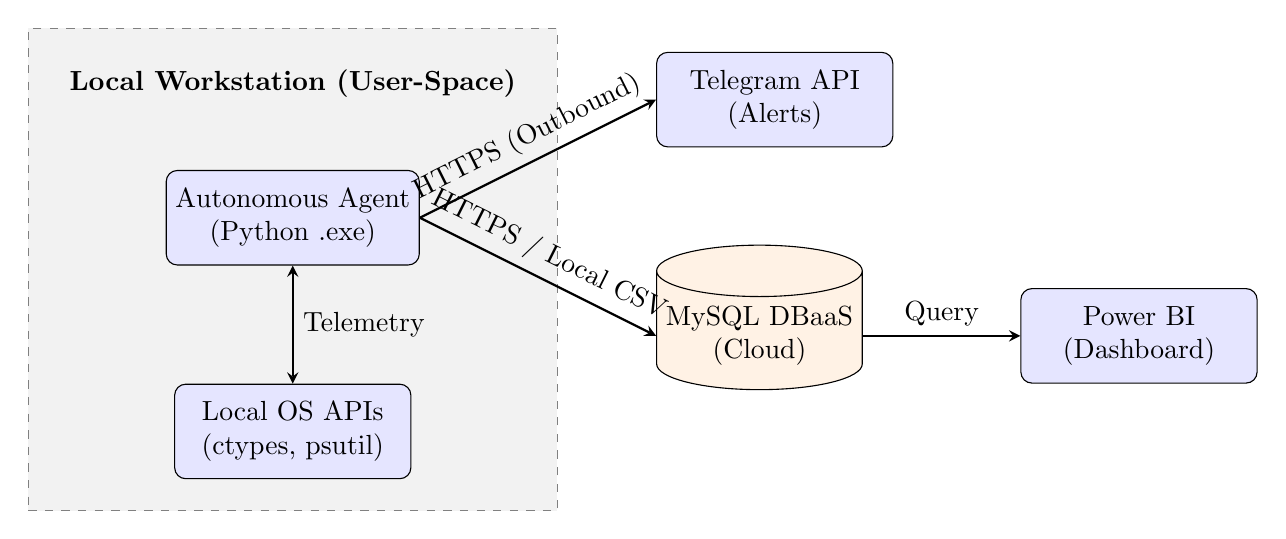
\begin{tikzpicture}[
    node distance=2cm and 3cm,
    box/.style={draw, rectangle, minimum width=3cm, minimum height=1.2cm, align=center, fill=blue!10, rounded corners},
    db/.style={draw, cylinder, shape border rotate=90, aspect=0.25, minimum height=1.5cm, minimum width=2.2cm, align=center, fill=orange!10},
    arrow/.style={->, >=stealth, thick}
]

\node[box] (agent) {Autonomous Agent \\ (Python .exe)};
\node[box, below=1.5cm of agent] (os) {Local OS APIs \\ (ctypes, psutil)};

\node[above=0.8cm of agent] (title) {\textbf{Local Workstation (User-Space)}};

\begin{scope}[on background layer]
    \node[fill=gray!10, draw=gray, dashed, fit=(title) (agent) (os), inner sep=0.4cm] (pc) {};
\end{scope}

\node[box, right=3cm of agent, yshift=1.5cm] (telegram) {Telegram API \\ (Alerts)};
\node[db, right=3cm of agent, yshift=-1.5cm] (mysql) {MySQL DBaaS \\ (Cloud)};
\node[box, right=2cm of mysql] (powerbi) {Power BI \\ (Dashboard)};

\draw[arrow, <->] (agent) -- node[right] {Telemetry} (os);
\draw[arrow] (agent.east) -- node[above, sloped] {HTTPS (Outbound)} (telegram.west);
\draw[arrow] (agent.east) -- node[above, sloped] {HTTPS / Local CSV} (mysql.west);
\draw[arrow] (mysql.east) -- node[above] {Query} (powerbi.west);

\end{tikzpicture}%
}
\caption{Decentralized Software-Defined System Architecture}
\label{fig:arch}
\end{figure}

To manage communication without violating perimeter network policies, the architecture implements unidirectional (Outbound) connections via the HTTPS protocol. The agent transmits critical alerts to a Telegram bot and stores historical status logs in a cloud-hosted MySQL database (DBaaS). As a redundancy and fault-tolerance mechanism against potential firewall blocks, the design includes the temporary persistence of logs in a local Comma-Separated Values (CSV) file. The final layer of the architecture consists of visualizing the collected data using Microsoft Power BI, enabling the generation of analytical savings reports without the need to develop a visualization system from scratch.

The operational design of the autonomous agent was formulated to mitigate the risk of academic data loss, a critical consideration in engineering environments where processes such as rendering or compiling frequently occur in the background without peripheral interaction. As illustrated in the operational flowchart in Fig. \ref{fig:flow}, the system logic performs a dual validation before executing any invasive action.

\begin{figure}[htbp]
\centering
\resizebox{\columnwidth}{!}{%
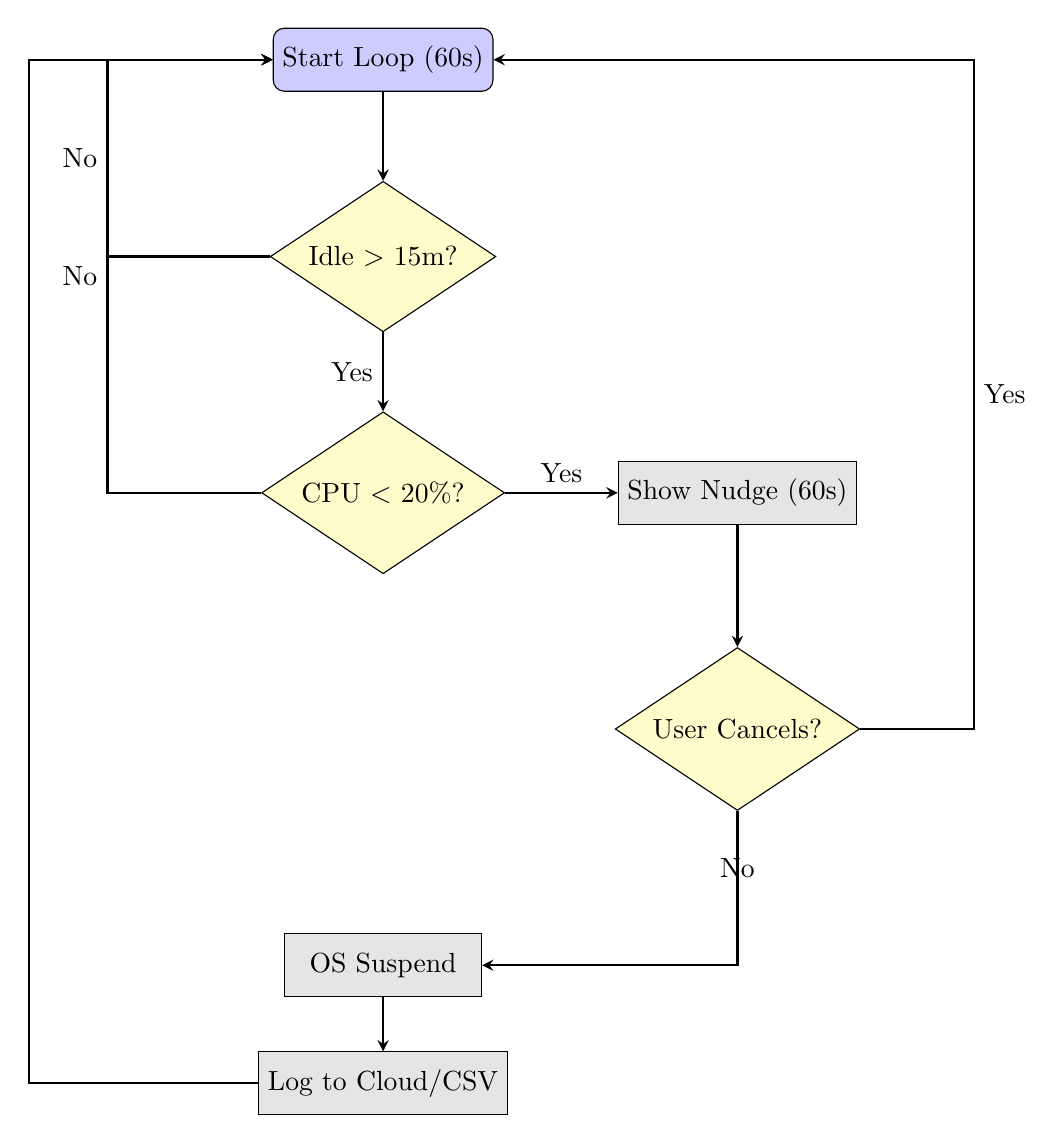
\begin{tikzpicture}[
    node distance=1.5cm,
    startstop/.style={rectangle, rounded corners, minimum width=2.5cm, minimum height=0.8cm, text centered, draw=black, fill=blue!20},
    process/.style={rectangle, minimum width=2.5cm, minimum height=0.8cm, text centered, draw=black, fill=gray!20},
    decision/.style={diamond, minimum width=2.5cm, minimum height=0.8cm, text centered, draw=black, fill=yellow!20, aspect=1.5},
    arrow/.style={thick,->,>=stealth}
]

\node (start) [startstop] {Start Loop (60s)};
\node (idle) [decision, below of=start, yshift=-1cm] {Idle $>$ 15m?};
\node (cpu) [decision, below of=idle, yshift=-1.5cm] {CPU $<$ 20\%?};
\node (nudge) [process, right of=cpu, xshift=3cm] {Show Nudge (60s)};
\node (cancel) [decision, below of=nudge, yshift=-1.5cm] {User Cancels?};
\node (suspend) [process, below of=cpu, yshift=-4.5cm] {OS Suspend};
\node (log) [process, below of=suspend] {Log to Cloud/CSV};

\draw [arrow] (start) -- (idle);
\draw [arrow] (idle) -- node[anchor=east] {Yes} (cpu);
\draw [arrow] (idle) -- ++(-3.5,0) |- node[anchor=east, near start] {No} (start);
\draw [arrow] (cpu) -- node[anchor=south] {Yes} (nudge);
\draw [arrow] (cpu) -- ++(-3.5,0) |- node[anchor=east, near start] {No} (start);
\draw [arrow] (nudge) -- (cancel);
\draw [arrow] (cancel) -- ++(3,0) |- node[anchor=west, near start] {Yes} (start);
\draw [arrow] (cancel) |- node[anchor=south, near start] {No} (suspend);
\draw [arrow] (suspend) -- (log);
\draw [arrow] (log) -- ++(-4.5,0) |- (start);

\end{tikzpicture}%
}
\caption{Agent Operational Workflow and Decision Logic}
\label{fig:flow}
\end{figure}

The agent enters an evaluation stage only if keyboard and mouse inactivity exceeds fifteen uninterrupted minutes. Subsequently, it corroborates that the current processor (CPU) load is below 20\%. Only when both conditions are affirmatively met does the software project a full-screen behavioral "nudge", requesting the occupant to interact with the machine if it is still in use. The absence of cancellation by the user within a sixty-second margin triggers the safe invocation of the operating system's native Sleep states, ensuring the preservation of the workspace while drastically interrupting the flow of electrical consumption.

\section{Results and Discussion}
The proposal for this system was configured as an academic Proof of Concept (PoC) that seeks to empirically validate the viability of digital behavioral intervention. With the designed architecture and established algorithms, the project sets up a battery of black-box experiments and projected performance metrics for the execution phase, which will allow contrasting the system's behavior against the human inertia detected in Phase 1 of the analysis.

The conceived unit and integration tests focus on evaluating the resilience of the Python agent against the injection of high computational demand background processes, ensuring the system does not incur false positives of inactivity. Table \ref{tab:metrics} consolidates the expected objective results for this PoC, establishing success thresholds centered on software availability, projected energy impact, and the end-user experience within the laboratories.

\begin{table}[htbp]
\caption{Proof of Concept Evaluation Metrics}
\label{tab:metrics}
\centering
\begin{tabular}{|p{2.5cm}|p{2cm}|p{3.5cm}|}
\hline
\textbf{Metric} & \textbf{Goal} & \textbf{Measurement Method} \\
\hline
Reliability & $>95\%$ Uptime & Deviation of generated logs vs. expected logs. \\
\hline
Energy Savings & $>20\%$ improvement & Hours in suspension multiplied by nominal consumption. \\
\hline
Intervention & $<10\%$ forced & Rate of canceled nudges vs. total suspensions. \\
\hline
False Positives & Zero (0) complaints & Reports of suspension during academic activities. \\
\hline
\end{tabular}
\end{table}

Unlike traditional home automation systems that require considerable investments and the replacement of electrical infrastructure, the analytical results suggest that this user-space software approach is superior in terms of cost-benefit for the university. The "nudge" strategy directly attacks the bottleneck identified in the surveys, transforming the device itself into an active educational agent that prevents negligence before applying the suspension. Although the energy-saving estimates must be mathematically validated after collecting the log files, the ability to deploy a monitoring network without escalating IT privileges constitutes a highly functional software design achievement.

\section{Conclusions}
This work comprehensively addressed the problem of inefficient energy consumption in university laboratories, demonstrating through systematic analysis that the main cause is the human factor and the normalization of waste in unoccupied spaces. Faced with institutional network and security blocks that disabled classic Internet of Things approaches, the design iterated towards an innovative solution: a Software-Defined Energy Management System.

By shifting the decision intelligence directly to the user-space of each workstation, the proposed design successfully circumvented physical infrastructure barriers. The decentralized architecture of the telemetry agents and the strategic use of behavioral intervention techniques demonstrated that obtaining granular control of sustainability on a campus is viable without compromising its cybersecurity or operational budgets. The next step in this research will involve executing the Proof of Concept in a controlled laboratory, collecting the empirical evidence needed in Power BI repositories to quantify the actual savings achieved in kilowatts.

\section*{Acknowledgments}
The authors extend their gratitude to Eng. Carlos Andrés Sierra and the Faculty of Engineering at Universidad Distrital Francisco José de Caldas for their theoretical training and for encouraging rigorous applied analysis and design of complex systems.

\begin{thebibliography}{00}
\bibitem{b1} M. V. Doblari, \textit{Gestión integral de energía en instituciones universitarias. Caso: Edificio Eva Duarte de Perón UNNOBA}, Master's Thesis, Universidad Nacional del Noroeste de la Prov. de Buenos Aires, Argentina, n.d.
\bibitem{b2} M. Abad Mier, \textit{Gestión energética de la biblioteca universitaria de la UVA, aplicando la ISO 50001}, Bachelor's Thesis, Universidad de Valladolid, Spain, 2015.
\bibitem{b3} J. C. Figueroa Sandrez, ``Gestión energética sostenible y su impacto en la huella de carbono: estudio de caso universitario,'' \textit{Journal of Management \& Business Studies}, vol. 7, 2025.
\bibitem{b4} B. Meza-Alcívar, M. Alemán-García, and M. Herrera-Suárez, ``Implementación de un sistema de gestión energético para institutos de educación superior,'' \textit{Revista Científica INGENIAR}, vol. 6, no. 12, 2023.
\bibitem{b5} O. Y. Fonseca López, D. F. Barrera Suárez, D. M. Ballesteros Molina, and D. L. Guzmán Triviño, ``Smart Campus Energy Management System,'' systems analysis, Universidad Distrital Francisco José de Caldas, Colombia, 2026.
\end{thebibliography}

\end{document}